% One forward pass of the frozen Electronic seed-0 model on test query 20, with its real numbers.
% Build: pdflatex forward.tex && pdftoppm -png -r 200 -singlefile forward.pdf forward
\documentclass[tikz,border=8pt]{standalone}
\usepackage{amsmath,amssymb}
\usetikzlibrary{arrows.meta,calc}
\definecolor{cC}{HTML}{7B4FB8}\definecolor{cL}{HTML}{1C9A8A}\definecolor{cG}{HTML}{3A8F3A}\definecolor{cS}{HTML}{C8372D}
\tikzset{
  arr/.style={-{Stealth[length=2.2mm]},line width=0.7pt,draw=black!60},
  box/.style={draw=black!55,fill=black!4,line width=0.7pt,rounded corners=3pt,align=left,font=\small,inner sep=5pt},
  term/.style={line width=0.7pt,rounded corners=3pt,align=left,font=\footnotesize,inner sep=5pt,text width=4.75cm,anchor=north west,minimum height=2.75cm},
  seed/.style={draw=black!60,fill=black!10,line width=0.7pt,rounded corners=3pt,align=left,font=\small,inner sep=5pt,text width=6.9cm},
  lab/.style={font=\small},
  tiny/.style={font=\scriptsize,text=black!60},
  stephead/.style={font=\bfseries\small,anchor=west},
}
% weighted contribution bars: \seg{row y}{start}{length}{colour}, one unit of score = \u cm
\def\uu{0.62}
\newcommand{\seg}[4]{\fill[#4] ({\zx+\uu*(#2)},{#1-0.2}) rectangle ({\zx+\uu*(#2+#3)},{#1+0.2});}
\begin{document}
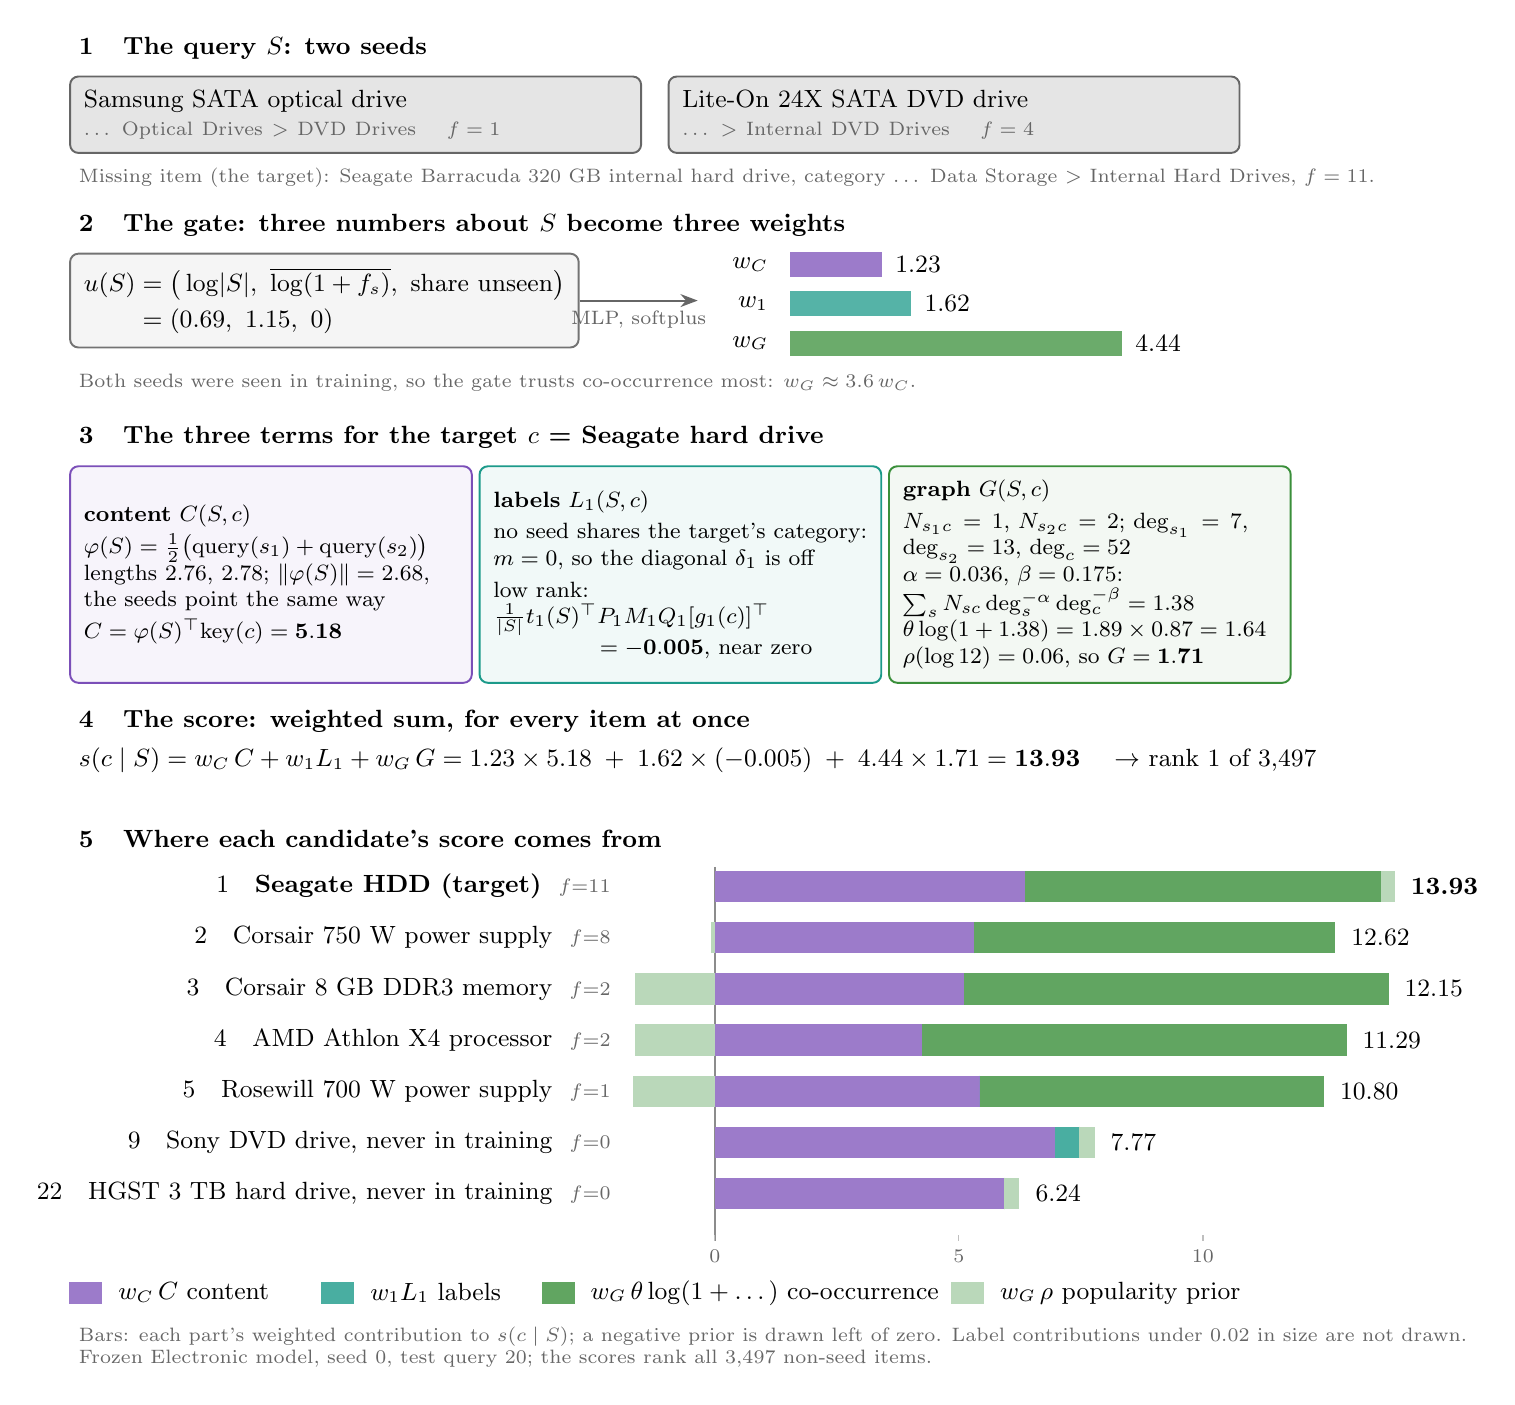
\begin{tikzpicture}[x=1cm,y=1cm]
% ------------------------------------------------------------------ step 1: the query
\node[stephead] at (0,0) {1\quad The query $S$: two seeds};
\node[seed,anchor=north west] (s1) at (0,-0.35) {Samsung SATA optical drive\\[-1pt]{\scriptsize \textcolor{black!60}{\dots\ Optical Drives $>$ DVD Drives \quad $f = 1$}}};
\node[seed,anchor=north west] (s2) at (7.6,-0.35) {Lite-On 24X SATA DVD drive\\[-1pt]{\scriptsize \textcolor{black!60}{\dots\ $>$ Internal DVD Drives \quad $f = 4$}}};
\node[tiny,anchor=west] at (0,-1.65) {Missing item (the target): Seagate Barracuda 320 GB internal hard drive, category \dots\ Data Storage $>$ Internal Hard Drives, $f = 11$.};
% ------------------------------------------------------------------ step 2: the gate
\node[stephead] at (0,-2.25) {2\quad The gate: three numbers about $S$ become three weights};
\node[box,anchor=north west] (u) at (0,-2.6) {$u(S) = \big(\log\lvert S\rvert,\ \overline{\log(1+f_s)},\ \text{share unseen}\big)$\\[2pt]
$\phantom{u(S)} = (0.69,\ 1.15,\ 0)$};
\draw[arr] (u.east) -- ++(1.5,0) node[midway,below,tiny]{MLP, softplus};
% weight bars
\foreach \name/\val/\col/\y in {$w_C$/1.23/cC/-2.75,$w_1$/1.62/cL/-3.25,$w_G$/4.44/cG/-3.75}{
  \node[lab,anchor=east] at (9.0,\y) {\name};
  \fill[\col!75] (9.15,{\y-0.16}) rectangle ++({0.95*\val},0.32);
  \node[lab,anchor=west] at ({9.2+0.95*\val},\y) {\val};}
\node[tiny,anchor=west] at (0,-4.25) {Both seeds were seen in training, so the gate trusts co-occurrence most: $w_G \approx 3.6\,w_C$.};
% ------------------------------------------------------------------ step 3: the three terms for the target
\node[stephead] at (0,-4.95) {3\quad The three terms for the target $c$ = Seagate hard drive};
\node[term,draw=cC,fill=cC!6] at (0,-5.3) {\textbf{content} $C(S,c)$\\[2pt]
$\varphi(S) = \tfrac12\big(\mathrm{query}(s_1)+\mathrm{query}(s_2)\big)$\\
lengths $2.76$, $2.78$; $\lVert\varphi(S)\rVert = 2.68$,\\the seeds point the same way\\[2pt]
$C = \varphi(S)^\top \mathrm{key}(c) = \mathbf{5.18}$};
\node[term,draw=cL,fill=cL!6] at (5.2,-5.3) {\textbf{labels} $L_1(S,c)$\\[2pt]
no seed shares the target's category:\\$m = 0$, so the diagonal $\delta_1$ is off\\[2pt]
low rank: $\tfrac{1}{\lvert S\rvert}t_1(S)^\top P_1 M_1 Q_1[g_1(c)]^\top$\\
$\phantom{low rank:} = \mathbf{-0.005}$, near zero};
\node[term,draw=cG,fill=cG!6] at (10.4,-5.3) {\textbf{graph} $G(S,c)$\\[2pt]
$N_{s_1c} = 1$, $N_{s_2c} = 2$; $\deg_{s_1} = 7$, $\deg_{s_2} = 13$, $\deg_c = 52$\\
$\alpha = 0.036$, $\beta = 0.175$:\\
$\sum_s N_{sc}\deg_s^{-\alpha}\deg_c^{-\beta} = 1.38$\\
$\theta\log(1+1.38) = 1.89 \times 0.87 = 1.64$\\
$\rho(\log 12) = 0.06$, so $G = \mathbf{1.71}$};
% ------------------------------------------------------------------ step 4: the score
\node[stephead] at (0,-8.55) {4\quad The score: weighted sum, for every item at once};
\node[lab,anchor=west] at (0,-9.05) {$s(c\mid S) = w_C\,C + w_1 L_1 + w_G\,G = 1.23 \times 5.18 \;+\; 1.62 \times (-0.005) \;+\; 4.44 \times 1.71 = \mathbf{13.93}$ \quad $\to$ rank 1 of 3{,}497};
% ------------------------------------------------------------------ step 5: contributions for seven candidates
\begin{scope}[yshift=-0.4cm]
\node[stephead] at (0,-9.65) {5\quad Where each candidate's score comes from};
\def\zx{8.2}
\draw[black!45,line width=0.5pt] (\zx,-10.0) -- (\zx,-14.75);
\foreach \t in {0,5,10}{\node[tiny] at ({\zx+\uu*\t},-14.95) {\t};\draw[black!25] ({\zx+\uu*\t},-14.75) -- ++(0,0.08);}
% rows: y, label; segments: content, labels, graph co-occurrence, prior (negative to the left of zero)
\newcommand{\row}[9]{% y, name, rank, f, wC*C, w1*L (positive part), wG*Gcooc, wG*prior, total
  \node[lab,anchor=east,align=right] at (7.0,#1) {#3\quad #2\ \ {\scriptsize\textcolor{black!60}{$f{=}#4$}}};
  \pgfmathsetmacro{\a}{#5}\pgfmathsetmacro{\b}{#6}\pgfmathsetmacro{\c}{#7}\pgfmathsetmacro{\d}{#8}
  \seg{#1}{0}{\a}{cC!75}\seg{#1}{\a}{\b}{cL!80}\seg{#1}{\a+\b}{\c}{cG!80}
  \ifdim \d pt>0pt \seg{#1}{\a+\b+\c}{\d}{cG!35}\else \seg{#1}{\d}{-\d}{cG!35}\fi
  \node[lab,anchor=west] at ({\zx+\uu*(\a+\b+\c+max(\d,0))+0.08},#1) {#9};}
\row{-10.25}{\textbf{Seagate HDD (target)}}{1}{11}{6.36}{0}{7.29}{0.28}{\textbf{13.93}}
\row{-10.9}{Corsair 750 W power supply}{2}{8}{5.31}{0}{7.40}{-0.07}{12.62}
\row{-11.55}{Corsair 8 GB DDR3 memory}{3}{2}{5.11}{0}{8.69}{-1.64}{12.15}
\row{-12.2}{AMD Athlon X4 processor}{4}{2}{4.25}{0}{8.69}{-1.64}{11.29}
\row{-12.85}{Rosewill 700 W power supply}{5}{1}{5.43}{0}{7.05}{-1.68}{10.80}
\row{-13.5}{Sony DVD drive, never in training}{9}{0}{6.96}{0.51}{0}{0.31}{7.77}
\row{-14.15}{HGST 3 TB hard drive, never in training}{22}{0}{5.93}{0}{0}{0.31}{6.24}
% legend
\foreach \col/\txt/\x in {cC!75/$w_C\,C$ content/0,cL!80/$w_1 L_1$ labels/3.2,cG!80/$w_G\,\theta\log(1+\dots)$ co-occurrence/6.0,cG!35/$w_G\,\rho$ popularity prior/11.2}{
  \fill[\col] (\x,-15.55) rectangle ++(0.42,0.28);\node[lab,anchor=west] at (\x+0.5,-15.41) {\txt};}
\node[tiny,anchor=west,align=left] at (0,-16.1) {Bars: each part's weighted contribution to $s(c\mid S)$; a negative prior is drawn left of zero. Label contributions under 0.02 in size are not drawn.\\Frozen Electronic model, seed 0, test query 20; the scores rank all 3{,}497 non-seed items.};
\end{scope}
\end{tikzpicture}
\end{document}
